\chapter{Les Œuvres Universitaires}

\section{Introduction}
    Notre projet comprend la conception et la réalisation d'une application d'aide à la gestion des ressources de la direction des œuvres universitaires (D.O.U) en général. Celle-ci offre des services de transport, de restauration, de bourse, d'hébergement et d'activités scientifiques, culturelles et sportives. Ces mêmes services lui ont été délégués par l'Office National des œuvres universitaires en fonction de la wilaya où est siégée cette même \acs{D.O.U}.\\
    
    À cet effet, il est nécessaire de présenter ces services en plus des missions la \acs{D.O.U} en tant qu'organisme d'accueil afin de comprendre leur principale activités.\\

\section{Présentation de la \acs{D.O.U} \cite{dou}}
    Les directions des œuvres Universitaires ont été créé conformément à l'arrêté interministériel du 22 décembre 2004 comportant la fixation de leurs sièges en plus de la liste constituant les résidences universitaires qui leur sont rattachées. Elles sont placées sous la tutelle de l'Office National des œuvres universitaires.\\

    Elles sont chargées de veiller à la gestion des ressources financières et humaines, du bon déroulement et du contrôle des résidences universitaires dont elles sont responsables, de la gestion du transport entre les résidences et les différents établissements de l'enseignement supérieur et de la restauration, de la wilaya dont elles font partie.\\

\section{Missions et activités de la \acs{D.O.U} \cite{onou-arrete}}
    Sa mission est de prendre en charge les différentes activités qui lui sont déléguées par l'Office National des œuvres universitaires qui est lui-même sous la tutelle du ministère de l'enseignement supérieur et de la recherche scientifique.\\
    
    Principalement organiser et gérer les services d'hébergement, de restauration, de bourse, de transport et activités scientifique, culturelles et sportives, de manière à assurer la satisfaction des besoins de l’étudiants.\\
    
    Plus précisément :
    
    \begin{itemize}\renewcommand{\labelitemi}{$\bullet$}
        \item Veiller à la gestion des moyens matériels et financiers qui lui sont affectés.
        \item Prendre les mesures nécessaires au bon fonctionnement des structures placées sous son autorité.
        \item Veiller à la gestion de son personnel et du personnel des résidences universitaires sous son autorité.
        \item Veiller au bon contrôle rationnelle des moyens mis a la disposition des résidences universitaires sous son autorité.
        \item S'assurer, avec les structures et organismes concernés, du suivi des opérations d'investissement et d'équipement des résidences universitaires sous son autorité.
        \item Soumettre périodiquement des rapports sur le fonctionnement des résidences universitaires sous son autorité.
        \item Participer à la création et au bon suivi de l'application du règlement intérieur des résidences universitaires sous son autorité.
        \item Approuver et suivre le bon déroulement des programmes d'activités scientifiques, culturelles et de loisirs des résidences universitaires sous son autorité.
        \item Passez tout marché et contrat en relation avec la restauration et le transport assuré par les résidences universitaires sous son autorité.
        \item Exercer l'autorité hiérarchique sur son personnel.
        \item Nommer les personnels dont le mode de nomination n'est pas prévu.
        \item Ordonner les crédits qui lui sont délégués.
    \end{itemize}

\section{L’organisation de la \acs{D.O.U} \cite{onou-arrete}}
    La direction des œuvres universitaires est composée de 04 départements selon le diagramme suivant :

    \begin{figure}[H]
        \centering
            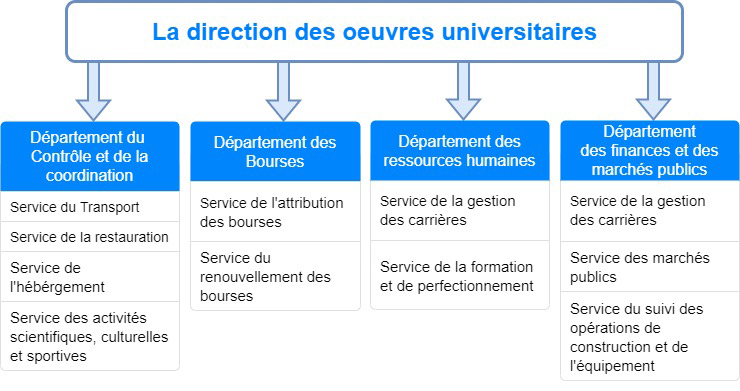
\includegraphics[scale=0.6]{chapitre1/direction-org.jpg}
        \caption{Organigramme de La Direction des Œuvres Universitaires}
    \end{figure}

    Chaque département regroupe plusieurs services qui sont chargé d'assurer différentes fonctions :

    \subsection{Le département du controle et de la coordination}
        \begin{itemize}
            \item Service du transport.
            \item Service de la restauration.
            \item Service de l'hébergement.
            \item Service des activités scientifiques, culturelles et sportives.\\
        \end{itemize}
        
        Ce département est chargé de :
        \begin{itemize}\renewcommand{\labelitemi}{$\bullet$}
            \item Mettre en œuvre les plans de transport universitaire des résidences universitaires rattachées à la \acs{D.O.U} et superviser le processus jusqu'à son aboutissement.
            \item Superviser, surveiller et orchestrer les actes d'œuvre universitaires assurées par les résidences universitaires associées à la \acs{D.O.U}.
            \item Présenter des méthodes rationnelles d'utilisation de tous les moyens dédiés aux activités des œuvres universitaires.
            \item Contrôler, et Assurer la bonne application des programmes d'activités scientifiques, et sportives approuvées par le directeur de la direction.
        \end{itemize}

    \subsection{Le département des ressources humaines}
        \begin{itemize}
            \item Service de la gestion des carrières.
            \item Service de la formation et de perfectionnement.\\
        \end{itemize}

        Ce département est chargé de :
        \begin{itemize}\renewcommand{\labelitemi}{$\bullet$}
            \item La gestion de la carrière du personnel de la \acs{D.O.U}.
            \item L'implémentation des plans de formation et perfectionnement du personnel de la \acs{D.O.U}.
        \end{itemize}

    \subsection{Le département des bourses}
        \begin{itemize}
            \item Service de l'attribution des bourses.
            \item Service du renouvellement des bourses.\\
        \end{itemize}
        
        Ce département est chargé de :
        \begin{itemize}\renewcommand{\labelitemi}{$\bullet$}
            \item Suivre et garantir le traitement des dossiers des étudiants bénéficiaires de bourses.
            \item Garantir le paiement régulier des bourses.
            \item Prendre en charge et garantir le traitement des bourses des étudiants étrangers.
        \end{itemize}

    \subsection{Le département des finances et des marchés publics}
        \begin{itemize}
            \item Service du budget et de la comptabilité.
            \item Service des marchés publics.
            \item Service du suivi des opérations de construction et de l'équipement.\\
        \end{itemize}

        Ce département est chargé de :
        \begin{itemize}\renewcommand{\labelitemi}{$\bullet$}
            \item Gérer les moyens matériels et financiers qui ont été mis à la disponibilité de la \acs{D.O.U}.
            \item Garantir de service de traitements des personnels de la \acs{D.O.U}.
            \item Garantir le contrôle des divers étapes de passation des marchés publics et d'en surveiller l'exécution par les résidences universitaires.
            \item Garantir, en conjonction avec les services concernés, la surveillance des actes de construction et d'équipement des résidences universitaires.\\
        \end{itemize}

\section{Analyse du système}
    La \acs{D.O.U} comprend donc quatre départements, département des bourses, département du contrôle et de la coordination, département des ressources humaines et le département des finances et des marchés publics.
    Parmi ces départements, Le département du contrôle et de la coordination se constitue lui-même de quatre services.\\

    Voici donc un récapitulatif des différentes taches dont ces services sont chargés d'exécuter et de veiller sur leurs bonne exécution:

    \subsection*{Hébérgement}
    Le service d'hébergement comprend deux sections, la section de l'attribution de l'hébergement et la section de la gestion. À se fait, ce service a pour tâches :

    \begin{itemize}
        \item Inscription des nouveaux bacheliers, et réinscription des anciens étudiants, ceci ce fait au niveau de chaque résidence.
        \item Contrôler les dossiers.
        \item Établir des statistiques sur l'état des résidences en rédigeant des listes globales de tous les étudiants et leurs répartitions par résidence et par bloc en tenant compte des nombres de places libres, les abandons, ... etc.
    \end{itemize}

    \subsection*{Transport}
    \begin{itemize}
        \item Assurer le transport des étudiants des résidences universitaires vers les campus pédagogiques en tenant compte du trajet inverse.
    \end{itemize}

    \subsection*{Réstauration}
    \begin{itemize}
        \item Assurer les repas au étudiants internes et externes.
    \end{itemize}

    \subsection*{Bourse}
    \begin{itemize}
        \item Assurer le traitement et le suivi des dossiers des étudiants bénéficiaires de bourses.
        \item Assurer le renouvellement des bourses.
        \item Assurer le paiement régulier des bourses.
        \item Assurer le traitement et la prise en charge des bourses des étudiants étrangers.\\
    \end{itemize}

Parmi les problèmes qui existent après l’analyse de ce système, on peut citer :
    \begin{itemize}
        \item Le transfert de données entre la \acs{D.O.U} et les différentes résidences se fait manuellement.
        \item La répartition des étudiants d’une manière arbitraire, ce qui engendre l’augmentation de l’enveloppe budgétaire alloue au transport.
        \item La perte de temps.
        \item La non disponibilité des informations au bon moment.
        \item La \acs{D.O.U} dispose d'un réseau informatique à haut débit mais très mal exploité. En fait, il n'existe aucune application ou logiciel fonctionnant sous réseau.
        \item La grande difficulté d'accéder aux informations en tant qu'étudiants. Les seules moyens qui existent actuellement sont des pages facebook, des photos de fiches mal prise et des sites internet existant mais qui ne marches pas et/ou ne contient pas les informations pertinente dont l'étudiant a besoin.
        \item La non existence des informations concernant les repas des services de restauration.
        \item L'inconsistance et l'incohérence des informations.\\
    \end{itemize}

\section{Présentation de la solution}
    Afin de remédier aux problèmes cités ci-dessus. Nous avons proposé de concevoir une application de gestion de ressources en se basant sur les Progiciels de Gestion Intégré \acs{ERP}, ceci pour permettre de :\\

    \begin{itemize}
        \item Informatiser l'ajout, la validation et le rejet des dossiers.
        \item Informatiser la liste des résidences et des campus universitaires.
        \item Automatiser la gestion des trajets du service des transports.
        \item Rendre public les informations sur les services de restauration et de transport notamment les menus des restaurants universitaires et les trajets des bus universitaires. 
        \item Informatiser l'affectation des étudiants aux résidences.
        \item Informatiser la gestion de la restauration, notamment les ingrédients, les plats, les menus et le calendrier des menus.
        \item Avoir une plateforme centraliser pour la gestion de tous les services du département du contrôle et de la coordination, voire plus.
        \item Avoir un rapport mensuel des menus, des ingrédients et des plats du service de la restauration.
        \item Avoir un rapport mensuel des trajets et des bus du service des transports.
        \item Normaliser et regrouper les informations concernant les \acs{D.O.U}.\\
    \end{itemize}

\section{Conclusion}
    Après avoir présenté l’organigramme d’accueil et différentes tâches accomplies par ces départements et leurs services nous avons remarqué que plusieurs de ces services souffre de multiples problèmes qui sont liés particulièrement à une mauvaise gestion des ressources en plus d’une retenue de l’information et le traitement manuel de l'information.\\

    Le chapitre suivant sera consacrée à la présentation des solutions de gestion de ressources et plus particulièrement a l'\acs{ERP}.

\newpage

\leftskip=0cm
\renewcommand{\bibname}{Référence bibliographique et webographique du chapitre 1}
\bibliographystyle{ieeetr}	
\bibliography{chapitre1/chap1}